
\chapter{Background and Related work}
\label{chap:related_works}

In recent years, the problem of text simplification has often been addressed as the monolingual language-to-language \emph{machine translation} from the original to simplified sentences. The existing machine translation models from the literature were modified to the particularities of the text simplification task.

\cite{zhu-etal-2010-monolingual} proposed a model for sentence simplification via \emph{tree transformation} based on the techniques from statistical machine translation. The model applies a sequence of simplification operations to perform splitting, dropping, reordering and word/phrase substitutions. 

A variation of \emph{phrase-based machine translation} (PBMT) with a dissimilarity component was proposed by \cite{wubben-etal-2012-sentence}. The proposed approach focuses on dissimilarity rather than deletion in the PBMT decoding stage, as simplification does not necessarily imply shortening. Outputs of the PBMT model are re-ranked according to their dissimilarity to the input sentence.

\cite{narayan-gardent-2014-hybrid} presented a hybrid approach to sentence simplification which combines \emph{deep semantics and monolingual machine translation} to derive simple sentences from the complex ones. Their simplification model consists of a probabilistic model for splitting and dropping, a PBMT model for substitution and reordering and a language model learned on Simple English Wikipedia for fluency and grammaticality. The simplification process is split into two steps. Firstly, the probabilistic model performs sentence splitting and deletion operations, therefore, producing one or more intermediate simplified sentences. Secondly, simplified sentences are further simplified using the PBMT system.

\begin{figure}[h]
    \centering
    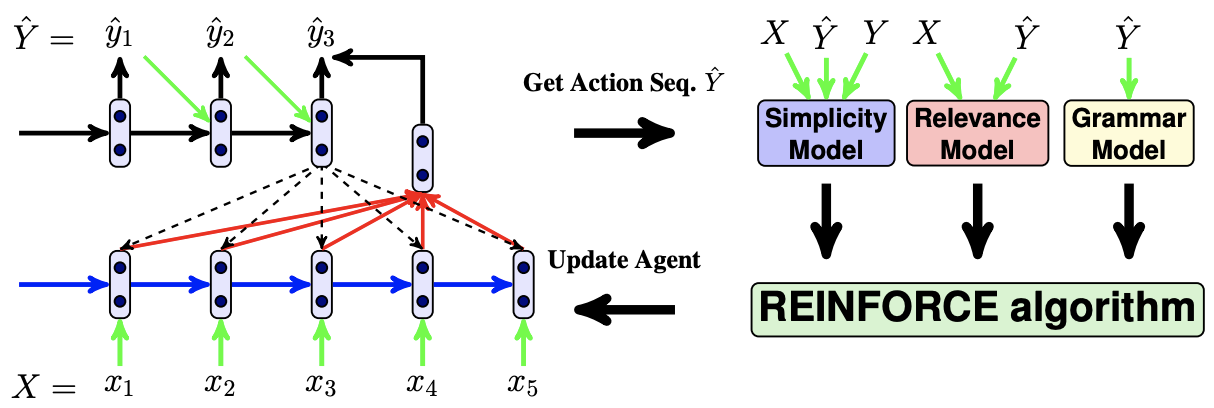
\includegraphics[width=14cm]{Images/dress.png}
    \caption{DRESS model. \textit{X} is the complex sentence, \textit{Y} is the reference sentence and \textit{$\hat{Y}$} simplification produced by the encoder-decoder model. Source: \cite{zhang-lapata-2017-sentence}.}
    \label{fig:dress}
\end{figure}

\cite{zhang-lapata-2017-sentence} proposed a \emph{deep reinforcement sentence simplification model} (DRESS, fig. \ref{fig:dress}) with an encoder-decoder architecture implemented by recurrent neural networks (RNNs). To make the output simpler and grammatically correct while also preserving the meaning of the input, they trained the model in a \emph{reinforcement learning} (RL) framework. It explores the space of possible simplifications while learning to maximize an expected reward function that encourages outputs that meets simplification constraints.

\section{Simplification as a style transfer}

Text simplification can be viewed as a form of \emph{style transfer} (\cite{wubben-etal-2012-sentence}; \cite{sulem-semantic-evaluation}), or \emph{stylistic paraphrasing}, with the goal of rewriting a sentence such that we preserve the meaning but alter the style. Generating paraphrases targeting a more general interpretation of style was first attempted in (\cite{xu-etal-2012-paraphrasing}). All of these works are based on statistical machine translation methods. 

Recently, however, the advances in neural machine translation have started to be applied to general stylistic paraphrasing. The Shakespeare dataset (\cite{xu-etal-2012-paraphrasing}) was used recently with a variation of Seq2Seq models (\cite{jhamtani-etal-2017-shakespearizing}). They proposed to use a mixture model of \emph{pointer network} and \emph{Long Short-Term Memory} (LSTM) to transform a modern English text to a Shakespearean style English. The authors reported an improvement over statistical machine translation methods. Another impressive work in this direction uses a large set of Bible translations to transfer a prose style with an encoder-decoder recurrent neural network and \emph{Moses} - a statistical machine translation system (\cite{carlson-bible}). Table \ref{tab:bible-style-transfer} gives some examples produced by this approach. 

\begin{table}[h]
\centering
\begin{tabular}{p{3.1cm}p{3.1cm}p{3.1cm}p{3.1cm}}
\hline
\textbf{Source} & \textbf{Target} & \textbf{Moses output} & \textbf{Seq2Seq} \\
\hline
Then Samuel gave him an account of everything, keeping nothing back. And he said, It is the Lord; let him do what seems good to him. & And Samuel told him every whit, and hid nothing from him. And he said, It is Jehovah: let him do what seemeth him good. & Then Samuel told him of all things not. And he said, It is Jehovah; let him do that which seemeth him good. & And Samuel told all things, and did not hold back. And he
said, It is Jehovah; let him do what seemeth good to him.\\
&&& \\
And Jehovah saith, 'Judah doth go up; lo, I have given the land into his hand'. & And the Lord said, Judah is to go up: see, I have given the land into his hands. & And the Lord said, 'Judah will go up, see, I have given the land into his hand.' & And the Lord said, Judah will go up; see, I will give the land into his hand.\\
\hline
\end{tabular}
\caption{Examples which show Moses and Seq2Seq Bible style transfer. Source: \cite{carlson-bible}.}
\label{tab:bible-style-transfer}
\end{table}

Unfortunately, the lack of appropriate training corpora has complicated the direct application of the style transfer approaches to text simplification.  

\section{Unsupervised style transfer}

In contrast, unsupervised style transfer algorithms work with unlabeled datasets which are significantly cheaper and easier to obtain. However, they are also considerably less explored in the literature. Amongst the few exceptions, are: 

\cite{Paetzold:2016:ULS:3016387.3016433} who proposed an unsupervised lexical simplification technique that replaces complex words in the input with simpler synonyms, which are extracted and disambiguated using word embeddings. 

\cite{Shen:2017:STN:3295222.3295427} who proposed to apply an \emph{adversarial training} to unsupervised style transfer and introduced a refined alignment of sentence representations across text corpora. They build an encoder that takes a sentence and its original style indicator as input and maps it to a style-independent content representation that is passed to a style-dependent decoder. The key contribution of this approach is in applying discriminators both on the encoder representation and on the hidden states of the decoders to ensure that they have the same distribution.

\cite{Zhang2018StyleTA} who proposed a two-stage joint training method to boost source-to-target and target-to-source style transfer systems using non-parallel text. They build bidirectional word-to-word style transfer systems in a statistical machine translation framework to generate a pseudo-parallel corpus and constructed two attention-based neural machine translation style transfer systems with the pseudo corpus. Then an iterative back-translation algorithm was employed to better leverage non-parallel text to jointly improve bidirectional neural machine translation based style transfer models.

\cite{surya-etal-2019-unsupervised} who used unlabeled corpora containing simple and complex sentences to train the system based on the shared encoder and two decoders. They proposed a novel training scheme which allows the model to perform content reduction and lexical simplification simultaneously through proposed losses and de-noising.

In comparison with the above-mentioned unsupervised models, we explore a novel application of the architecture for cross-lingual language modeling to the task of text simplification. Our approach achieves superior BLEU and SARI results on the Wikilarge dataset. In addition, we conduct a more comprehensive evaluation and assess the system's performance from a wider variety of metrics (see Chapter \ref{chap:methodology} and \ref{chap:experiments} for details).


\section{From LSTM to Transformers}
\label{sec:from_lstm_to_transformers}

More generally, the recent trend in natural language processing research has been around using \emph{Transformer} neural network architectures which are based on \emph{attention mechanisms} (\cite{NIPS2017_7181}). Thus, \cite{Radford2018}, \cite{howard-ruder-2018-universal} and \cite{Devlin2019BERTPO} investigated language modeling for pre-training Transformer encoders and demonstrated dramatic improvements on classification tasks from the GLUE benchmark (\cite{wang-etal-2018-glue}). \cite{ramachandran-etal-2017-unsupervised} showed that machine translation tasks can also gain significant improvements by utilizing language modeling pre-training.

\cite{zhao2018integrating} introduced a supervised sentence simplification model based on the Transformer architecture and proposed two approaches to integrating the Simple PPDB (\cite{pavlick-callison-burch-2016-simple}) knowledge base for simplification that contains 4.5 million paraphrase rules. The first one is the \emph{Deep Memory Augmented Sentence Simplification} (DMASS) model. It has an augmented dynamic memory to record multiple key-value pairs for each rule in the Simple PPDB which helps to overcome the problem when the neural network focuses more on frequent rules and ignores rare rules. The second model, \emph{Deep Critic Sentence Simplification} (DCSS), encodes the context and the output of each simplification rules into the shared parameters. 

\cite{Mikolov2013ExploitingSA}, \cite{Faruqui2014ImprovingVS}, \cite{Xing2015NormalizedWE} and \cite{Ammar2016MassivelyMW} investigated usage of small dictionaries to align \emph{word representations} from different languages. The need for cross-lingual supervision was slashed by \cite{DBLP:journals/corr/SmithTHH17} and completely removed by \cite{conneau2017word}.

\bigskip
Numerous works on the text simplification task prove once again its importance. Recent advances in the field of NLP have been dictated by \textit{Transfer Learning} methods with Transformer language models. They became the source of our inspiration for this work and we believe they can rise text simplification systems to a new level.

\endinput